% History
% 12/06/2024  (岸)	修論下書き用texファイル作成
% 12/12/2024  (岸)	フォントサイズを11pt, 行間を1.5に設定
% コンパイルの仕方
% 		uplatex chapter1_v1.tex
% 		upbibtex chapter1_v1
% 		uplatex chapter1_v1.tex
% 		uplatex chapter1_v1.tex
% 		dvipdfmx chapter1_v1.dvi

% フォントサイズを11ptに設定
\documentclass[a4paper,11pt,nomag]{jsreport}

\usepackage[dvipdfm,truedimen]{geometry}
\geometry{top=22mm,bottom=22mm,left=22mm,right=22mm}
%% jsclasses系で文字サイズ11pt や 12pt をクラスオプションに指定すると,
%% 長さが拡大されるため,nomagオプションを併用している.
%% https://oku.edu.mie-u.ac.jp/~okumura/jsclasses/ のFAQをよく読むこと.

%\usepackage{layout}
%\usepackage[utf8]{inputenc} %不要かも
\usepackage[T1]{fontenc} %utf8フォントエンコーディング指定
\usepackage{lmodern} % 11pt, nomag を使っているので
% CloudLaTeX の場合は下の1行を有効にすること
% \AtBeginDvi{\special{pdf:mapfile ptex-ipaex.map}}
\usepackage{array}
\newcommand{\bhline}[1]{\noalign{\hrule height #1}}  
\newcommand{\bvline}[1]{\vrule width #1}
\renewcommand{\baselinestretch}{1.5} % 教授が赤修正を入れやすいように行間を1.5に設定
\usepackage[subrefformat=parens]{subcaption}
\usepackage[dvipdfmx]{graphicx} % dvipdfmx を前提としている
\usepackage[dvipdfmx]{color}
\usepackage{caption}
\usepackage{subcaption}
\usepackage{bbm}
\usepackage{multirow}
\usepackage{arydshln}
\usepackage{here} % 図表の位置決め用
\usepackage{amsmath,amssymb}% 数式用
\usepackage{url}      % URL等記載用.\verbより便利
\usepackage{enumerate}
\usepackage{midpage}

% サブキャプションのフォーマットを調整
\renewcommand\thesubfigure{(\alph{subfigure})}
\captionsetup[subfigure]{labelformat=simple, labelsep=space}

\begin{document}
\setcounter{chapter}{3}

\chapter*{メタ学習に基づくInfrared Few-shot Open-set Recognitionを考慮した動物分類}

\section{未登録クラスに対する多クラス分類の高精度化に向けたクラスタリングに基づく損失関数}

\subsection{メタ学習にクラスタリングを導入する狙い}
既存のOSRやFSOSRは,未登録クラスの検出に取り組んでいるため,多クラス分類に適した特徴空間の構築が十分に行われていなかった.
これに対しIFORでは,未登録クラスに対する多クラス分類精度の向上に焦点を当てている.
% そこで,我々は,メタ学習にクラスタリングを導入し,未登録クラスの多クラス分類精度の向上を目指しました.
% ではなぜ,多クラス分類を意識した特徴空間の構築に対して,我々はクラスタリングに基づく損失が有効と考えたのか,その理由について説明します.
図 \ref{fig:feature_space}は,学習時における特徴空間上の各クラス分布を示す2つの例である.
% 
\begin{figure}[tbp]
  \centering
  \begin{subfigure}[b]{0.45\linewidth}
    \centering
    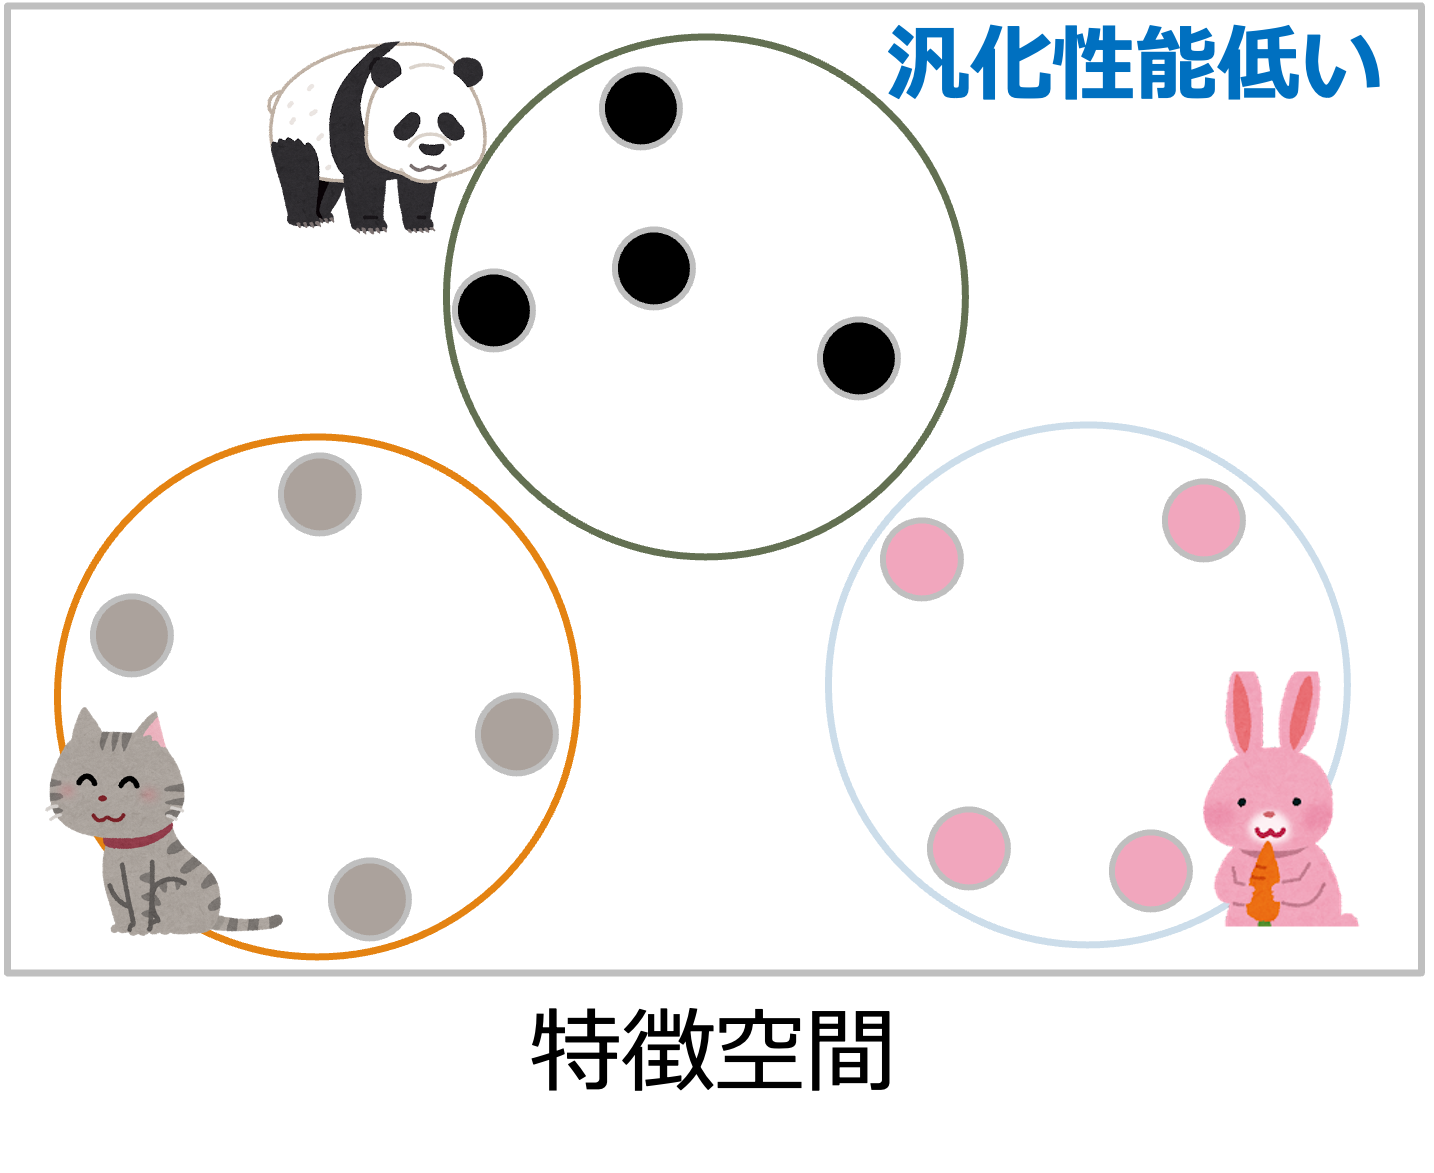
\includegraphics[height=0.9\linewidth, keepaspectratio]{image/bad_featurespace.png}
    \caption{汎化性能の低い特徴空間の例}
    \label{fig:bad_featurespace}
  \end{subfigure}
  \hfill
  \begin{subfigure}[b]{0.45\linewidth}
    \centering
    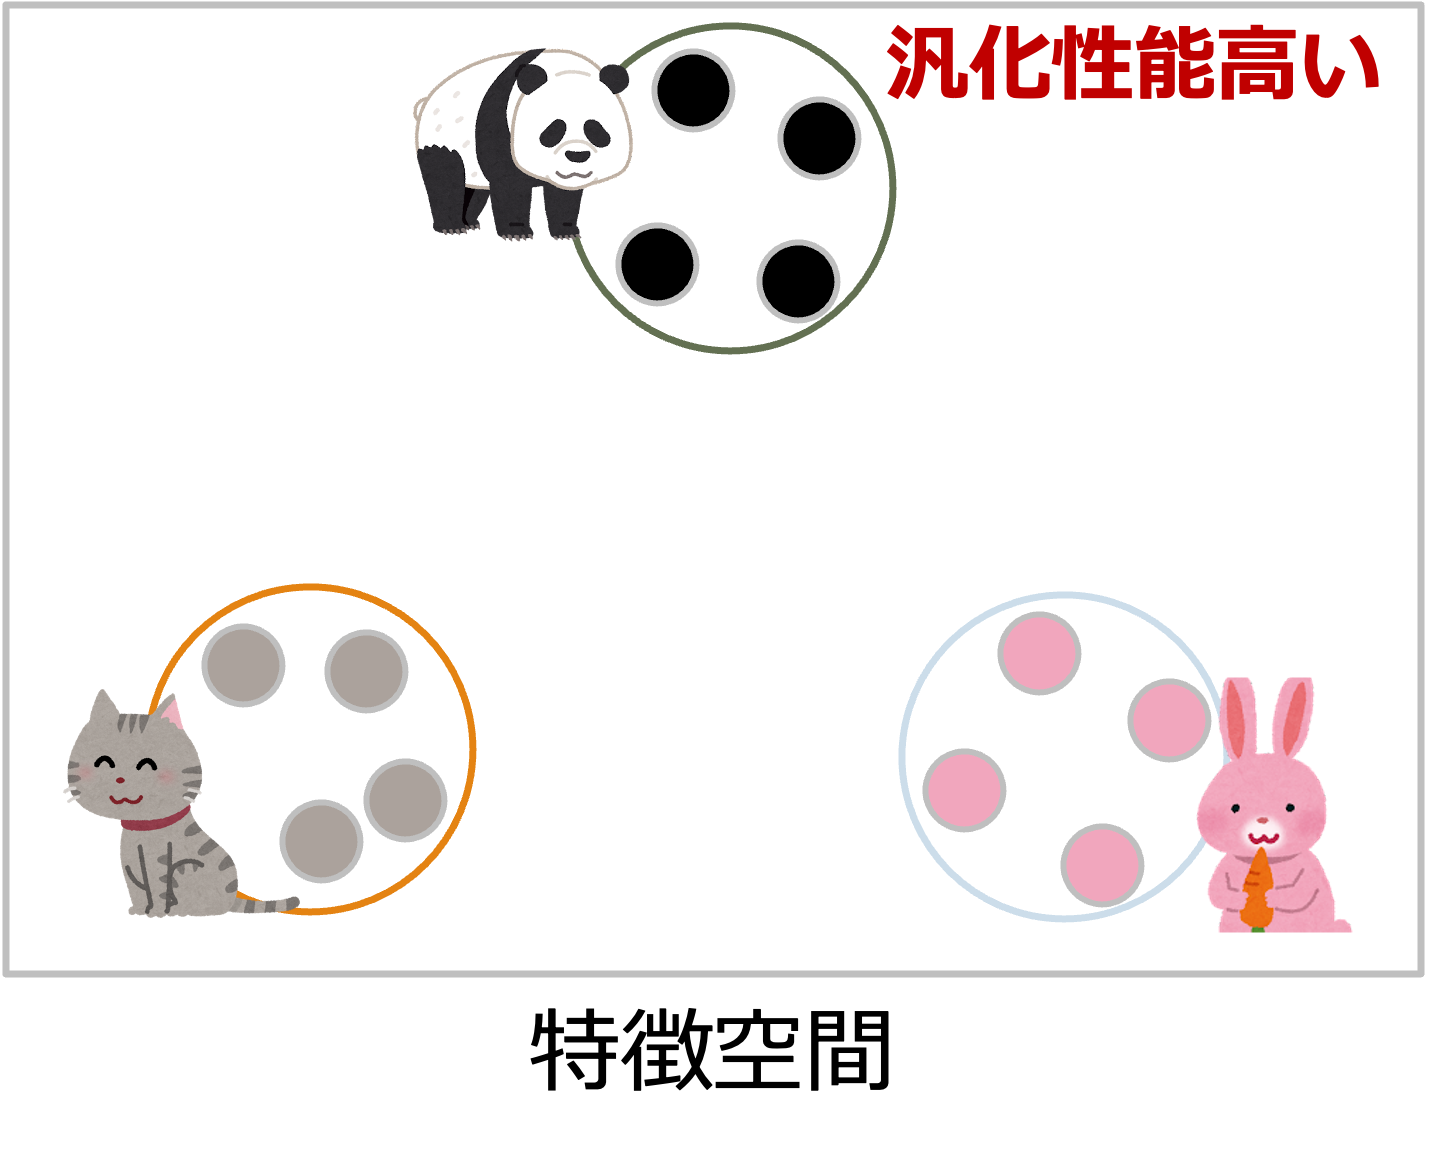
\includegraphics[height=0.9\linewidth, keepaspectratio]{image/good_featurespace.png}
    \caption{汎化性能の高い特徴空間の例}
    \label{fig:good_featurespace}
  \end{subfigure}
  \caption{学習時における特徴空間上の各クラス分布の例}
  \label{fig:feature_space}
\end{figure}
% 
図 \ref{fig:bad_featurespace}および図 \ref{fig:good_featurespace}に示された特徴空間はいずれも同程度の分類精度であるが,ドメインシフトなどを考慮した場合,図 \ref{fig:good_featurespace}の特徴空間の方が,新規地域に対する高い汎化性能を有していると考えられる.
これは,図 \ref{fig:good_featurespace}の方がクラス内分散が小さく,クラス間分散が大きいため,より高い表現力を有しており,新規地域における特徴抽出においても分類が容易となるような特徴空間の構築が期待できるからである.
したがって,本研究では,メタ学習にクラスタリングに基づく損失を導入することによって,クラス内分散の最小化・クラス間分散の最大化を実現し,IFORにおける未登録クラスの多クラス分類精度の向上を目指す.

\subsection{損失関数}

本研究では,FSL損失,OSR損失,分類損失に加え,k-means損失と Between-Class損失 (BC損失) を導入する.
k-means損失は,Chinら \cite{k-means}が異常検知タスクにおいて提案した損失であり,k-meansクラスタリングによって集約される類似した性質を持つ特徴量から,より優れた特徴表現を学習する.
k-means損失による学習の例を図 \ref{fig:kmeans_loss}に示す.
% 
\begin{figure}[tbp]
  \centering
  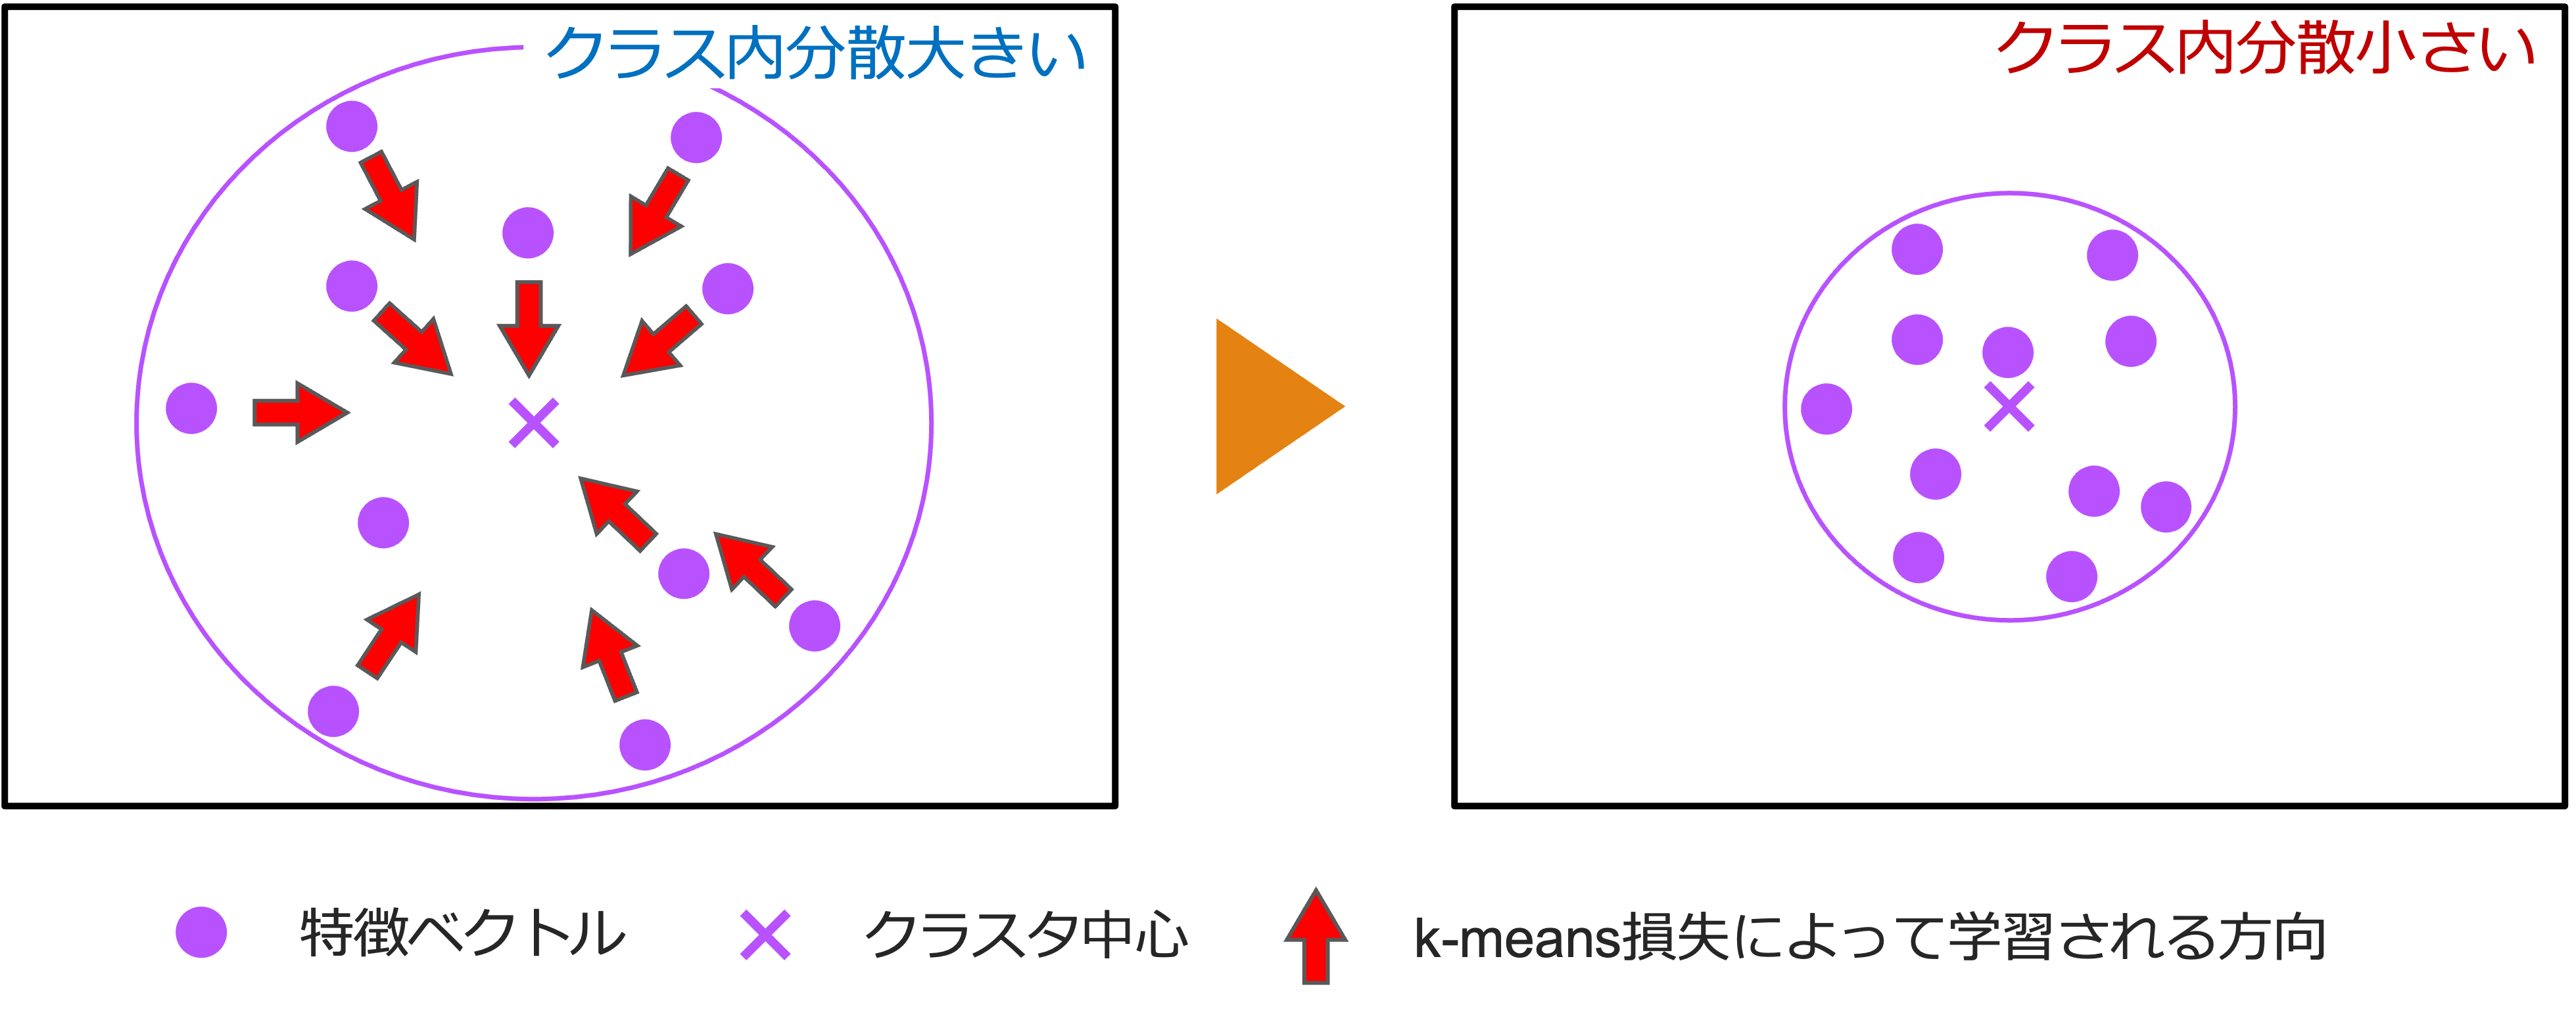
\includegraphics[width=\linewidth, keepaspectratio]{image/kmeans_loss.png}
  \caption{k-means損失によってクラス内分散が小さくなる例}
  \label{fig:kmeans_loss}
\end{figure}
% 
この損失関数では,同一クラスタ内の特徴ベクトルがクラスタ中心に可能な限り近接することが期待される.
本研究では,類似した性質を持つ特徴量のクラスタリングにより,特徴空間上の各クラスのクラス内分散を最小化することを目指し,k-means損失の有効性を検証する.
IFORフレームワークにおいて,k-means損失は以下のように定義される.

\begin{align}
\mathcal{L}_{Kmeans} = \sum_i{\min_k \lVert f(x_i)-c_k \rVert_2}
\end{align}

\noindent
ここで,$f(x_i)$は$i$番目の入力画像を特徴抽出器$f(\cdot)$に入力した際の特徴量,$c_k$は$k$番目のクラスタ中心を表す.

一方,BC損失は,クラス分布のコンパクトな表現に加え,各クラスの分布が可能な限り離れているような特徴空間の構築が,多クラス分類性能の向上に寄与するという考えに基づいている.
BC損失による学習の例を図 \ref{fig:bc_loss}に示す.
% 
\begin{figure}[tbp]
  \centering
  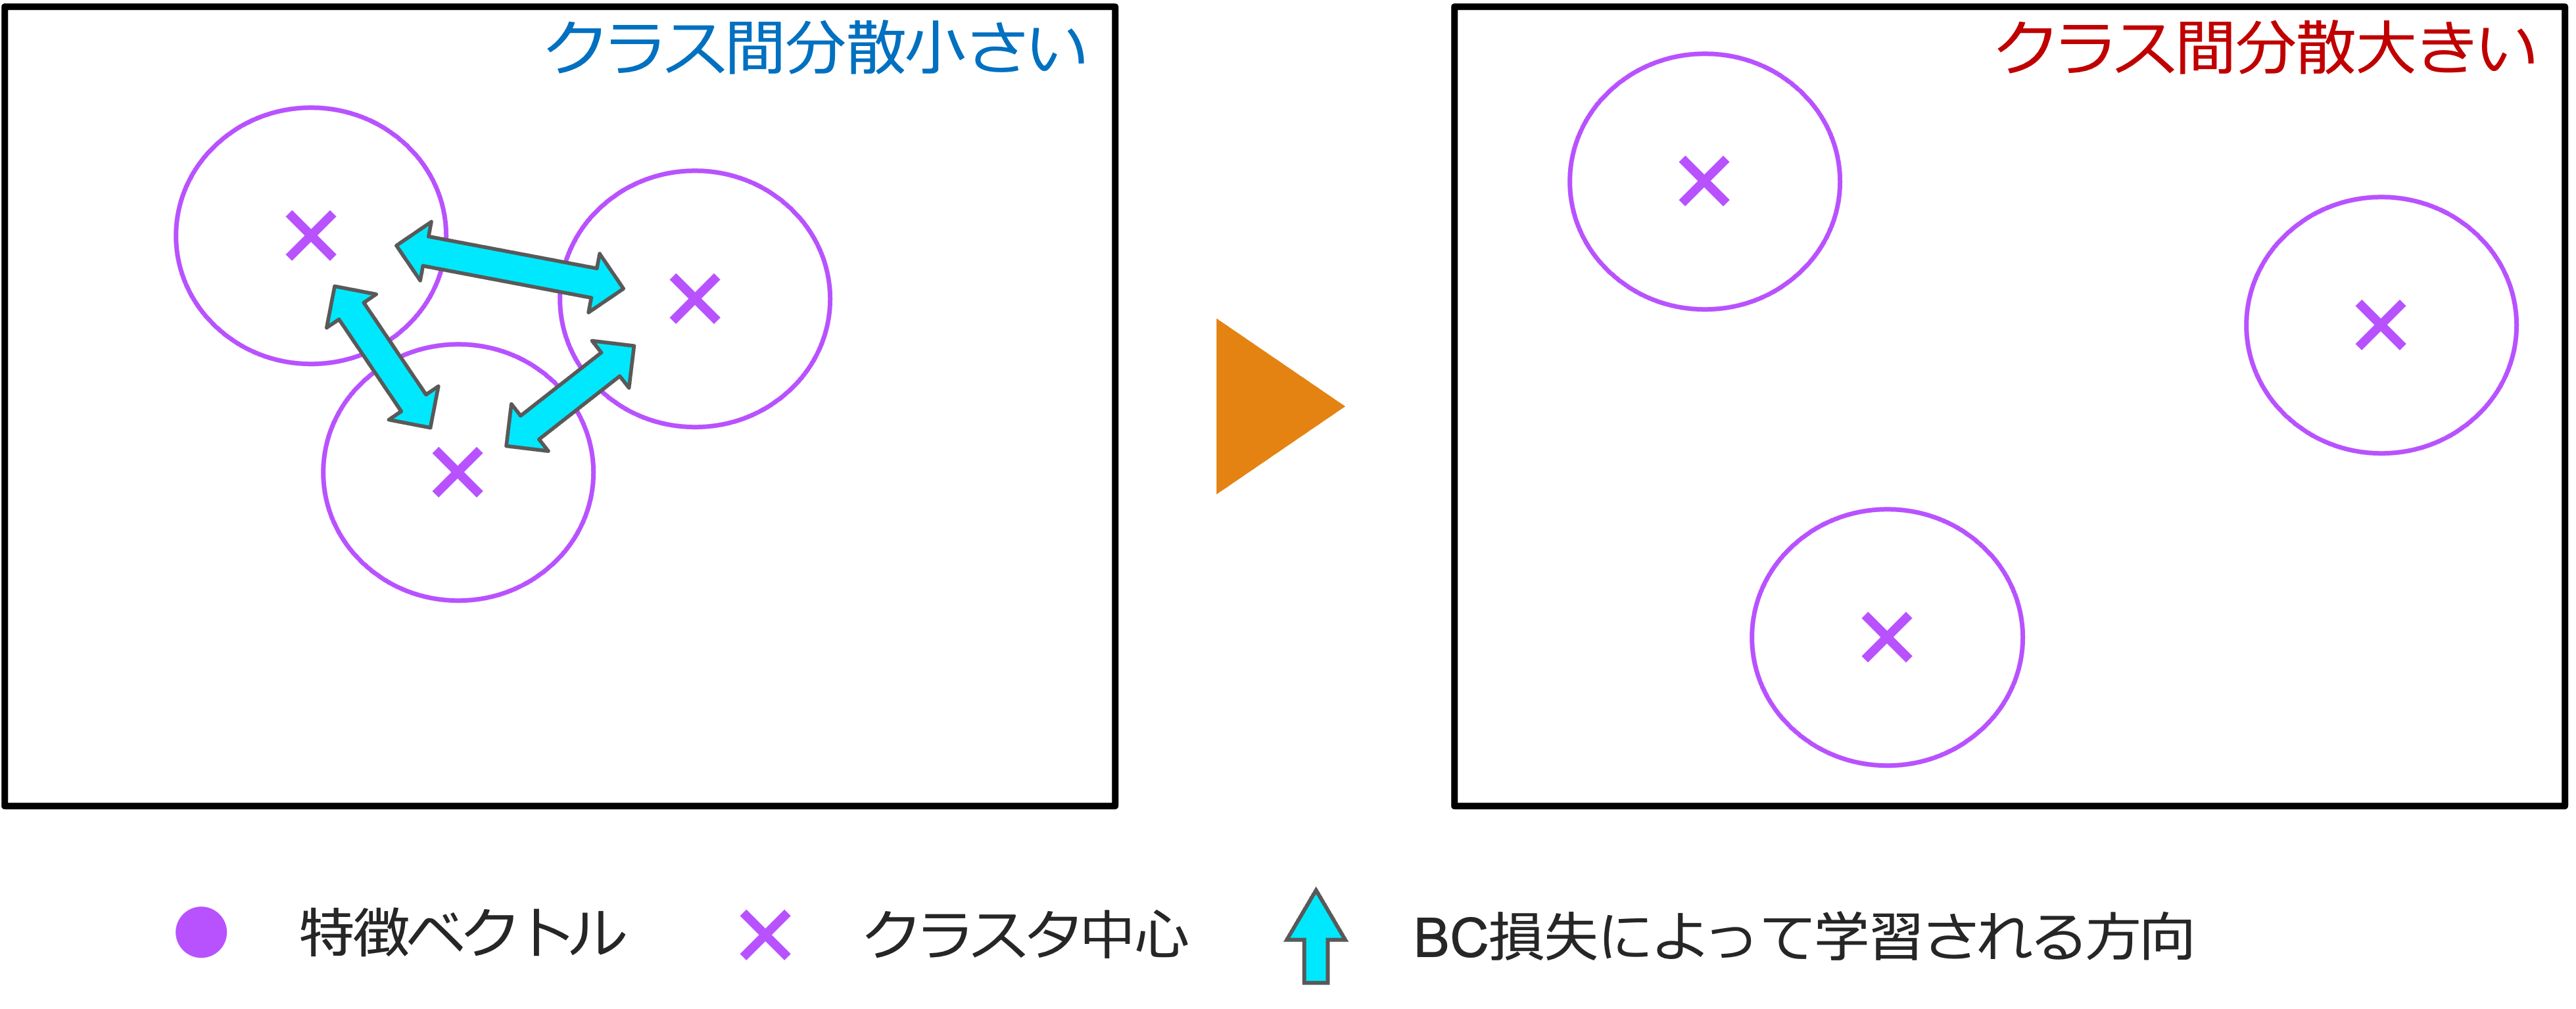
\includegraphics[width=\linewidth, keepaspectratio]{image/bc_loss.png}
  \caption{Between-Class損失によってクラス間分散が大きくなる例}
  \label{fig:bc_loss}
\end{figure}
%
この損失関数では,k-meansクラスタリングによって得られる各クラスタ中心間の距離を最大化することにより,クラス間分散の最大化を目指す.
IFORフレームワークにおいて,BC損失は以下のように定義される.

\begin{align}
  \mathcal{L}_{\text{Between-Class}} = -\log{\sum_{k_1} {\sum_{k_2} {\lVert c_{k_1} - c_{k_2} \rVert_2}}}
\end{align}

\noindent
ここで,$c_{k_1}$と$c_{k_2}$は$k_1$番目,$k_2$番目のクラスタ中心を表す.
負の符号を付与することにより,クラス間分散の最大化問題を損失関数の最小化問題として扱っている.

% ここから参考文献bibtexの設定
\bibliographystyle{../kishiIEEEtr}
\bibliography{../references}

\end{document}